\section{绪论}

\subsection{信号的概念}
信号\footnote{指电信号}是\uwave{信息的载体}

辨析:
\begin{itemize}
    \item 消息:人们常常把来自外界的各种报道统称为消息。
    \item 信息\footnote{本课程中对“信息”和“消息”两词不加严格区分}:通常把消息中有意义的内容称为信息。
    \item 信号:信号是信息的载体,通过信号传递信息。
\end{itemize}

\subsection{系统的概念}

\begin{Figure}[系统组成]
    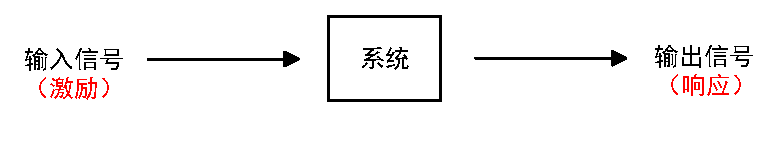
\includegraphics[width=100mm]{visio/1.1.pdf}
\end{Figure}

信号处理:对信号进行加工/变换

信号传输:通信(长距离)


